%%
\vspace{-1mm}
\section{Stateless Tracking}
\label{sec:stateless-tracking}

%%
\vspace{-2mm}
\subsection{Browser Fingerprinting}
\label{sec:browser-fingerprinting}
\vspace{-2mm}

%%
Browser (or device) fingerprinting is a technique used to collect information on users’ browsers and devices. 
%
By using HTTP headers and calling specific JavaScript API endpoints, a website can collect a wide range of information on the browser and its configuration (\eg{} browser version, screen size, installed list of fonts, GPU model, timezone and preferred languages) to the underlying operating system and the hardware. 
%
Research has shown that the diversity of Internet-connected devices is so vast that the combination of collected attributes can be unique, leading to the identification of a specific device~\cite{eckersleyHowUniqueYour2010, laperdrixBeautyBeastDiverting2016,gomez-boixHidingCrowdAnalysis2018}. 
%
\autoref{fig:stateless-tracking} depicts how fingerprinting works.
%
Analysis of real-world fingerprints and entropy computations of all attributes have revealed that some attributes contribute a lot more to the uniqueness of users than others. 
%
Entropy~\cite{bacis2024assessing} measures the level of uncertainty or unpredictability in a dataset to understand how varied its distribution can be. 
%
For example, if a device's screen size can have 8 distinct values, its entropy is 3 bits.
%
Unlike techniques described in~\autoref{sec:stateful-tracking}, fingerprinting: 
%
1) does not rely on a stored state (\ie{} ID) in the browser to track a user as the fingerprint collection is performed in real-time to identify a device; 
%
2) is hard to detect and block; 
%
3) is also difficult to evade as users keep the same device for months or years, resulting in stable fingerprints over time.

\begin{figure}[htbp]
    \vspace{-2mm}
    \centering
    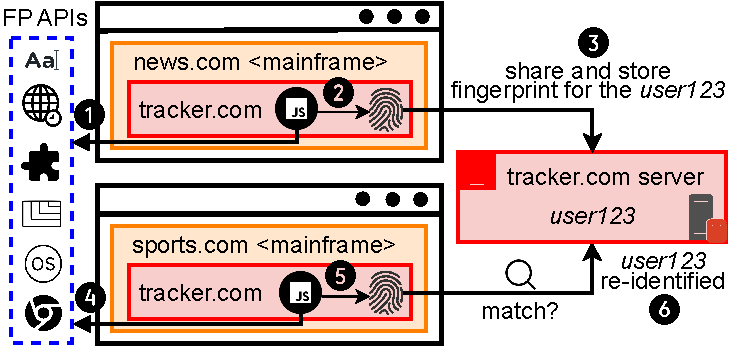
\includegraphics[width=0.8\linewidth]{figures/tracking-mechanisms-fingerprinting.pdf}
    \caption{Stateless Tracking via Browser Fingerprinting}
    \label{fig:stateless-tracking}
    \vspace{-2mm}
\end{figure}

%%
Since the first academic work on browser fingerprinting in 2009~\cite{mayerAnyPersonPamphleteer2009}, researchers have studied: its impact on privacy~\cite{eckersleyHowUniqueYour2010}, use with other tracking techniques~\cite{fouadMyCookiePhoenix2022}, its detection~\cite{iqbalFingerprintingFingerprintersLearning2021, boussahaFPtracerFinegrainedBrowser2024}, use in real world applications~\cite{aminazadWebRunner20492020, wuHimManyFaces2023}, abusable browser APIs~\cite{bahramiFPRadarLongitudinalMeasurement2022, suAutomaticDiscoveryEmerging2023, senolDoubleEdgedSword2024}, and user protections~\cite{vastelFpScannerPrivacyImplications2018}. 
%
In 2013, fingerprinting was observed on just $\sim$1\% of the top 10K websites~\cite{nikiforakisCookielessMonsterExploring2013} and $\sim$400 of the top 1 million websites~\cite{acarFPDetectiveDustingWeb2013}. 
%
Over the years, a variety of techniques have been used to measure browser fingerprinting~\cite{acarWebNeverForgets2014,englehardtOnlineTracking1millionsite2016,olejnikBatteryStatusNot2017,dasWebsSixthSense2018}, with two general trends being: its higher adoption by third-parties and its expansion to a diverse set of browser APIs over the years. 
%
By 2021, fingerprinting scripts were found to be present on 10\% of the top 100K websites, with more popular ones having a higher incidence (\ie{}, 30\% of the top 1,000)~\cite{iqbalFingerprintingFingerprintersLearning2021}.
%
Importantly, browser fingerprints are not always stable enough to track users over time: 80\% of browser instances change fingerprints in less than 10 days~\cite{vastelFPSTALKERTrackingBrowser2018}. 
%
Trackers not only link fingerprints as they evolve, but also combine and persist them with \textit{stateful} techniques, rendering effectiveness even in browsers that partition third-party access to stateful APIs (\autoref{sec:stateful-defenses}). 
%
A 2022 study showed a lower bound on this by detecting it on 1,150 of the top 30K sites~\cite{fouadMyCookiePhoenix2022}.
%
Other recent works indicate that fingerprinting risks differ across demographics~\cite{berkeHowUniqueWhose2025} and that limiting the information contained in fingerprints would not break the user experience~\cite{intumwayaseUARadarExploringImpact2023}.


%%
\vspace{-2mm}
\subsection{Types of Fingerprinting}
\label{sec:types-of-fingerprinting}
\vspace{-3mm}


%%
Besides browser fingerprinting techniques, researchers have demonstrated numerous side-channel approaches to track users.
%
One such approach is extension fingerprinting, aimed at inferring the presence of specific extensions in user's browser~\cite{karamiCarnusExploringPrivacy2020}. 
%
Early studies~\cite{sjostenDiscoveringBrowserExtensions2017, gulyasExtendNotExtend2018, karamiCarnusExploringPrivacy2020} demonstrated how extensions contain specific resources (\eg{}, images, scripts) that can be referenced by web pages, thereby revealing their presence in the user's browser. 
%
Researchers have also explored behavioral extension fingerprinting~\cite{starovXHOUNDQuantifyingFingerprintability2017, karamiCarnusExploringPrivacy2020, solomosDangersHumanTouch2022, solomosEscapingConfinesTime2022, laperdrixFingerprintingStyleDetecting2021, agarwalPeekingWindowFingerprinting2024}---where an extension can be implicitly inferred through executional side-effects---and corresponding mitigations~\cite{karamiUnleashSimulacrumShifting2022, sanchez-rolaExtensionBreakdownSecurity2017} such as randomizing WARs, IDs, or classes~\cite{trickelEveryoneDifferentClientside2019} and access control based extension loading~\cite{sjostenLatexGlovesProtecting2019}. 


%%
Apart from extension fingerprinting, prior works have explored various browser-supported JavaScript APIs for fingerprinting such as Canvas~\cite{moweryPixelPerfectFingerprinting2012}, WebGL~\cite{caoCrossBrowserFingerprintingOS2017}, Audio API~\cite{englehardtOnlineTracking1millionsite2016}, and the Battery Status API~\cite{olejnikLeakingBatteryPrivacy2016}. 
%
Sanchez-Rola et al. further demonstrated how JavaScript APIs can be used to construct a hardware fingerprint by analyzing the execution timing of instruction sequences~\cite{sanchez-rolaClockClockTimeBased2018}, while others have demonstrated browser-based fingerprinting techniques that target the device's CPU~\cite{trampertBrowserBasedCPUFingerprinting2022,matyuninTrackingPrivateBrowsing2018} or GPU~\cite{laorDRAWNAPARTDevice2022}. 
%
Recent research also demonstrates DRAM-based device fingerprinting capabilities from the vantage point of browsers~\cite{venugopalanFPRowhammerDRAMBasedDevice2024}.
%
Hardware-related fingerprints have also been extensively explored within the mobile ecosystem~\cite{bojinovMobileDeviceIdentification2014,dasTrackingMobileWeb2016,marcantoniLargescaleStudyRisks2019,hupperichRobustnessMobileDevice2015,deyAccelPrintImperfectionsAccelerometers2014,zhang2019sensorid}, due to the availability of additional sensors (\eg{}, gyroscope, magnetometer) which can exhibit unique hardware ``imperfections'' that occur during the manufacturing process. 
%
More broadly, any browser mechanism that extracts some form of data or affects client-side policies or behavior without storing a user-specific identifier, should be treated as a potential stateless tracking vector and analyzed accordingly~\cite{aliNavigatingMurkyWaters2023}. 
%
Generally, side-channel attacks are challenging to detect and could be equally difficult to mitigate.


%%
\vspace{-1mm}
\subsection{Need for Fingerprinting}
\label{sec:need-for-fingerprinting}
\vspace{-2mm}

%%
Constructively, fingerprinting can be thought of as a form of intrusion detection. 
%
Web applications can learn about the browsing environment of their first-party users and associate it with specific user identities~\cite{LinPhishSheepsClothing2022}. 
%
For example, a website can learn that the user Alice is using a smartphone with specific dimensions or a desktop browser with a specific kind of GPU. 
%
If Alice's credentials are ever stolen and an attacker attempts to login to that service, the service can extract the attacker's fingerprint, observe a major difference against Alice's fingerprints from prior sessions, and request additional authentication data from the attacker (such as a one-time password).
%
The same techniques can be constructively used to differentiate real users from malicious bots, as well as attackers engaging in ad fraud.


%%
Destructively, the same techniques that can identify user-impersonating attackers and bots, can be turned against users who wish to keep their identity anonymous. 
%
Using fingerprinting, a web application may be able to determine that a certain anonymous user is in fact eponymous, since their browser fingerprint matches that of a known user on the same platform. 
%
This undesired re-identification occurs despite user's attempt to hide by deleting their cookies or using the browser's private mode. 
%
In a cross-site context, fingerprinting can be abused to link unrelated website visits together, even when third-party cookies are disabled.


%%
\vspace{-1mm}
\subsection{Defenses Against Stateless Tracking}
\label{sec:stateless-defenses}
\vspace{-2mm}

%%
Browser vendors consider fingerprinting as a form of covert tracking that’s harmful to the web~\cite{nottinghamUnsanctionedWebTracking2015}. 
%
All major browsers have deployed some mitigations against fingerprinting and the W3C encourages specification authors to consider how their APIs contribute to the fingerprinting surface of the browser~\cite{dotyMitigatingBrowserFingerprinting2019}. 
%
Despite this, major browsers continue to expose a significant amount of information that can be used to fingerprint users.
%
There is no optimal strategy against fingerprinting as it often comes at the cost of user's utility. 
%
There is rather a disagreement between vendors on the feasibility of completely mitigating fingerprinting and the value of deploying incremental improvements without a clear path to complete mitigation~\cite{snyderBraveFingerprintingPrivacy2019, rescorlaTechnicalCommentsPrivacy2021}. 
%
% As such, fingerprinting mitigations vary greatly across browsers.

%%
The most common approach to mitigating fingerprinting is the normalization of device information exposed by browsers to reduce the utility of fingerprints. 
%
Browsers such as Tor make all users appear to have the same fingerprint, thereby making it hard to differentiate between them~\cite{perryDesignImplementationTor2013}. 
%
Whereas others introduce randomness so that a single user's fingerprint keeps changing from page load to page load, complicating user tracking. 
%
These latter countermeasures are easier to deploy across user populations and hence more popular than the ones which aim to make all environments appear identical.
%
Browser vendors have reduced identifying information exposed by APIs already shipped to the web, have removed web APIs known to be abused for fingerprinting, and have declined to implement new APIs that expose additional fingerprinting surfaces. 
%%
Examples include: freezing the minor browser version from the User-Agent string~\cite{weissIntentDeprecateFreeze2020}, unshipping the Battery Status API due to being fingerprintable~\cite{olejnikBatteryStatusNot2017}, and WebKit and Firefox’s refusal to implement the Network Information API, in part, due to fingerprinting concerns~\cite{TrackingPreventionWebKit2020, thomsonNetworkInformationAPI2018}.


%
Web API normalization sometimes breaks websites that expect to have access to device information. 
%
% For example, Mozilla rolled back their effort to freeze the Android OS version in Firefox for Android’s User-Agent string due to breakage on a major authentication provider~\cite{peterson1865766FreezeAndroid2024}. 
%
For web APIs that can’t be normalized, browsers have added site-specific randomized noise to the outputs of those APIs, for example, noise added to the rasterized outputs of the 2D Canvas, to WebGL renderings, and \texttt{AudioBuffer} samples from the WebAudio API. 
%
Randomization was first deployed by Brave under the name ``farbling’’~\cite{braveprivacyteamFingerprintingDefenses202020}, and was later adopted by Firefox~\cite{huang1816056FprandomizationMeta2023} and Safari~\cite{wilanderPrivateBrowsing202024}. Crucially, alternative fingerprinting techniques can still be employed~\cite{linFashionFauxPas2023}.


%%
Besides changes to individual API outputs, browsers have also explored approaches grounded in policy to discourage fingerprinting. 
%
Mozilla released an anti-tracking policy which forbids browser fingerprinting~\cite{mozillaSecurityTrackingPolicy2019} and subsequently blocked scripts from loading in Firefox when they were detected to include browser fingerprinting code~\cite{englehardtFirefox72Blocks2020}. 
%
Google Chrome engineers proposed a \textit{Privacy Budget} on websites where websites would be allowed to access fingerprintable device information up to a browser-defined budget~\cite{lasseyMikewestPrivacybudget2019}.
%
Once that budget is exceeded, the browser would limit the further exposure of identifying information. 
%
This approach was met with skepticism due to a likelihood of website breakage and risk of exposing additional tracking surface~\cite{snyderBraveFingerprintingPrivacy2019, rescorlaTechnicalCommentsPrivacy2021}, resulting in its discontinuation~\cite{leflerWhatHappenedPrivacy2024}. 
%
Thus, a lack of unified effort in the past decade to tackle fingerprinting suggests that, as of now, there is no desire in the tech community to remove it entirely. 